\documentclass[]{article}

%Deutsche Bezeichnungen für angezeigte Namen (z.B. Innhaltsverzeichnis etc.)
\usepackage[ngerman]{babel}

% prints dummy text
\usepackage{blindtext}

% Ränder bei Bedarf zeigen
%\usepackage{showframe}

%Erlaubt unteranderem Umbrücke captions
\usepackage{caption}

%Kompakte Listen
\usepackage{paralist}

%Zitate besser formatieren und darstellen
\usepackage{epigraph}

%Zeilenabstand 1,5
\usepackage[onehalfspacing]{setspace}

%Verbesserte Darstellung der Buchstaben zueinander
\usepackage[stretch=10]{microtype}

%Unterstützung von Umlauten und anderen Sonderzeichen (UTF-8)
\usepackage{lmodern}
\usepackage[utf8]{luainputenc}
\usepackage[T1]{fontenc}

%Einfachere Zitate
\usepackage{epigraph}

%Verwendung von Akronymen
\usepackage[printonlyused]{acronym}

%Unterstützung der H positionierung (keine automatische Verschiebung eingefügter Elemente)
\usepackage{float} 

%Erlaubt Umbrüche innerhalb von Tabellen
\usepackage{tabularx}

%Erlaubt Seitenumbrüche mit Tabellen
\usepackage{longtable}

%Erlaubt die Darstellung von Sourcecode mit Highlighting
\usepackage[outputdir=out]{minted}

%Definierung eigener Farben bei nutzung eines selbst vergebene Namens
\usepackage[table,xcdraw]{xcolor}

%Vektorgrafiken
\usepackage{tikz}

%Grafiken (wie jpg, png, etc.)
\usepackage{graphicx}

%Grafiken von Text umlaufen lassen
\usepackage{wrapfig}

%Ermöglicht Verknüpfungen innerhalb des Dokumentes (e.g. for PDF), Links werden durch "hidelink" nicht explizit hervorgehoben
\usepackage[hidelinks, ngerman]{hyperref}

%Einbindung und Verwaltung von Literaturverzeichnissen
\usepackage{csquotes} %wird von biber benötigt
\usepackage[style=alphabetic, backend=biber, bibencoding=utf8]{biblatex}
\addbibresource{references/references.bib}

% for enumeration
\usepackage{enumitem}

%-------------------------------Zusätzliche Anpassungen und Modifikationen--------------------------------------------%
%Pluszeichen in der Referenz beim zitieren ausblenden
\renewcommand*{\labelalphaothers}{}

\addto{\captionsngerman}{\renewcommand{\abstractname}{Abstract}}

%Exposé Type
\newcommand*{\exposeType}[1]{\gdef\@exposeType{#1}}

%%Exposé Type (CHOOSE ONE)
\exposeType{Bachelorabschlussarbeit}
%\exposeType{Masterabschlussarbeit}
%\exposeType{Forschungsprojekt A}
%\exposeType{Forschungsprojekt B}

\title{\bf Exposé - \@exposeType:\protect\\ Untersuchungen von Style Transfer Methoden für die Verwendung mit Leistungsarmer Hardware}
\author{Christoph Stach}
\date{07.01.2019}

\begin{document}

\maketitle

\begin{otherlanguage}{ngerman}
	\begin{abstract}
		Die Abschlussarbeit im Bereich der Angewandte Informatik handelt darum verschiedene Style Transfer Methoden zu implementieren,
		die Konzepte zu verstehen und Sie auf Tauglichkeit für Systeme mit leistungsarmer Hardware zu testen. Style Transfer ist eine Bereich des 
		Deeplearnings. Es werden dabei zwei willkürliche Bilder zu einem neuen Bild kombiniert. Beim ersten Bild wird der Inhalt aus dem Bild herausgefiltert,
		z.B. aus einem Foto auf dem ein Vogel zu sehen ist. Aus dem zweiten Bild wird Stil herausgefiltert, z.B. aus einem abstrakt gezeichneten Gemäden von Vincent van Gogh.
		Als Ergebnis entsteht ein neues Bild, welches den gleichen Vogel darstellt, als wäre er von Vincent van Gogh gemalt worden. 
		Es sollen unterschiedliche Algorithmen untersucht werden und die Ergebnisse mit einander vergleichen werden.
	\end{abstract}
\end{otherlanguage}

\section{Motivation}
TODO

\section{Zielsetzung}
Ziel des Projektes ist eine Anwendung zu erstellen die in der Lage ist
Style Transfer auf Geräten mit leistungsarmer Hardware (z.B. Mobiltelefonene oder Laptops ohne GPU) zu ermöglichen.

\section{Vorgehen}
Beispiel Angabe einer Quelle: Backpropagation Algorithm \cite{doi:10.1162/neco.1989.1.4.541}

\section{Erfordernisse und Randbedingungen}
Da das Berechnen von Deep Neural Networks und Convolutional Neural Networks sehr rechenintensiv sein kann,
werden diese normalerweise auf Serversystemen mit eingebauter Graphic Processing Unit realisiert. Das soll bei der Evaluation der 
Modelle berücksichtigt werden, damit Ergebnisse in einem vertretbaren Zeitaufwand auf Systemen ohne GPU entstehen.

\section{Zeitplan}
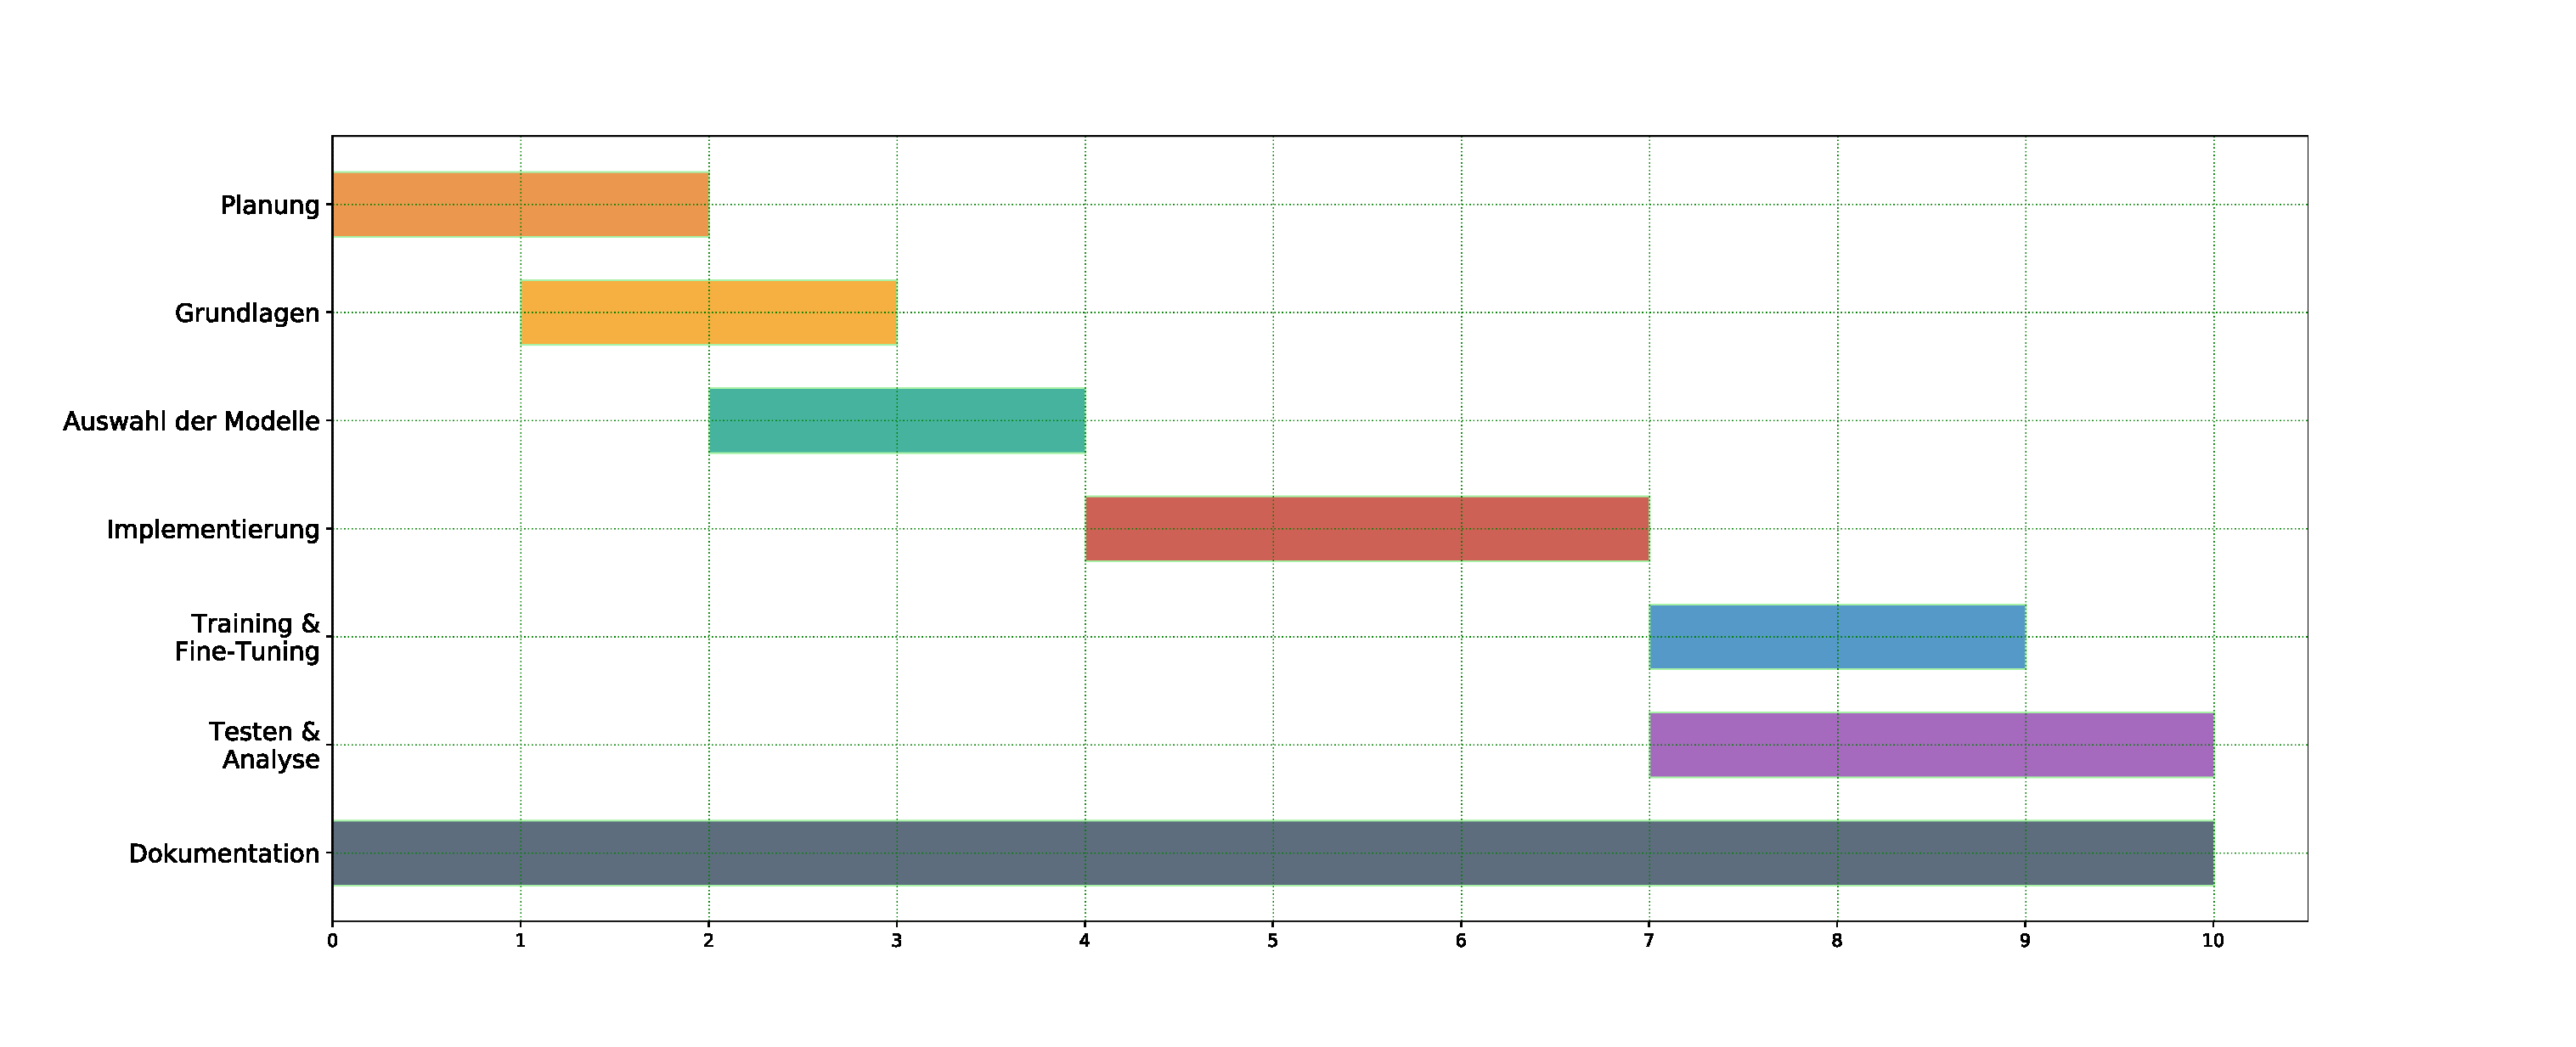
\includegraphics[width=1.00\textwidth]{resources/gantt.eps}
Das Gantt-Diagramm stellt den vorläufigen Zeitplan des Projektes da.
Dieser kann sich jedoch während des Projektverlaufes noch ändern und wird bei Bedarf angepasst.
Besonders zu beachten ist, dass das Training eines Neural Networks in Verbindung mit Großendatenmengen viel Zeit in Anspruch nehmen kann.
Deswegen wurden für das Training vorläufig zwei Wochen veranschlagt.

\section{Erwartete Ergebnisse}
Das Ergebnis des Projektes ist der laufähige Prototyp einer Anwedung mit mit der dazugehörigen Dokumentation und Erklärung
aller der Verwendeten Algorithmen und Modelle.

\section{Vorläufige Gliederung}

\begin{enumerate}
	\item Zusammenfassung (Abstract)
	\item Einleitung
	\item Grundlagen
	\item Analyse
	\item Konzeption
	\begin{enumerate}[label*=\arabic*.]
		\item Beispiel Unterkapitel
	\end{enumerate}
	\item Implementierung
	\item Test
	\item Evaluation
	\item Fazit / Ausblick
\end{enumerate}

\defbibfilter{scientific}{
	type=article or
	type=inbook or
	type=book or
	type=unpublished or
	type=inproceedings or
	type=incollection or
	type=manual or
	type=phdthesis
}

\printbibliography[heading=bibintoc, filter=scientific, title={Literaturangaben}]

\end{document}
